\documentclass[aspectratio=169]{beamer}

% Thème et configuration
\usetheme{Madrid}
\usecolortheme{default}

% Packages
\usepackage[utf8]{inputenc}
\usepackage[T1]{fontenc}
\usepackage[french]{babel}
\usepackage{graphicx}
\usepackage{booktabs}
\usepackage{array}
\usepackage{multirow}
\usepackage{tikz}
\usepackage{pgfplots}
\pgfplotsset{compat=1.18}

% Configuration des couleurs
\definecolor{univ_blue}{RGB}{0,84,159}
\definecolor{tech_green}{RGB}{46,125,50}
\definecolor{accent_orange}{RGB}{255,152,0}

\setbeamercolor{structure}{fg=univ_blue}
\setbeamercolor{frametitle}{bg=univ_blue,fg=white}
\setbeamercolor{title}{fg=univ_blue}

% Informations du document
\title[Reconnaissance Caractères Ourdou]{Reconnaissance de Caractères Ourdou avec Deep Learning}
\subtitle{Approche Progressive du MLP aux CNN Profonds}
\author[A. VITOFFODJI]{Adjimon VITOFFODJI}
\institute[Paul Valéry]{
    Master MIASHS \\
    Université Paul Valéry, Montpellier III
}
\date{Juin 2025}

% Configuration de la navigation
\setbeamertemplate{navigation symbols}{}
\setbeamertemplate{footline}[frame number]

% Commandes personnalisées
\newcommand{\emphasize}[1]{\textcolor{accent_orange}{\textbf{#1}}}
\newcommand{\accuracy}[1]{\textcolor{tech_green}{\textbf{#1}}}

\begin{document}

% Page de titre
\begin{frame}
    \titlepage
    \vspace{-0.5cm}
    \begin{center}
        \small Challenge Kaggle : IST Deep Learning Workshop \\
        \vspace{0.3cm}
        \tiny Tuteur : M. Jérôme Pasquet
    \end{center}
\end{frame}

% Plan de présentation
\begin{frame}{Plan de Présentation}
    \tableofcontents
\end{frame}

\section{Contexte et Objectifs}

\begin{frame}{Contexte du Projet}
    \begin{columns}[T]
        \begin{column}{0.6\textwidth}
            \textbf{Challenge Kaggle :} IST Deep Learning Workshop
            
            \vspace{0.5cm}
            \textbf{Objectif Principal :}
            \begin{itemize}
                \item Classifier \emphasize{40 caractères ourdou} distincts
                \item Images 28×28 pixels en niveaux de gris
                \item Optimiser la précision de classification
            \end{itemize}
            
            \vspace{0.5cm}
            \textbf{Motivation :}
            \begin{itemize}
                \item Préservation du patrimoine linguistique
                \item \emphasize{170+ millions} de locuteurs ourdou
                \item Défis spécifiques aux langues non-latines
            \end{itemize}
        \end{column}
        \begin{column}{0.4\textwidth}
            % Remplacez par votre image
            \begin{figure}
                \centering
                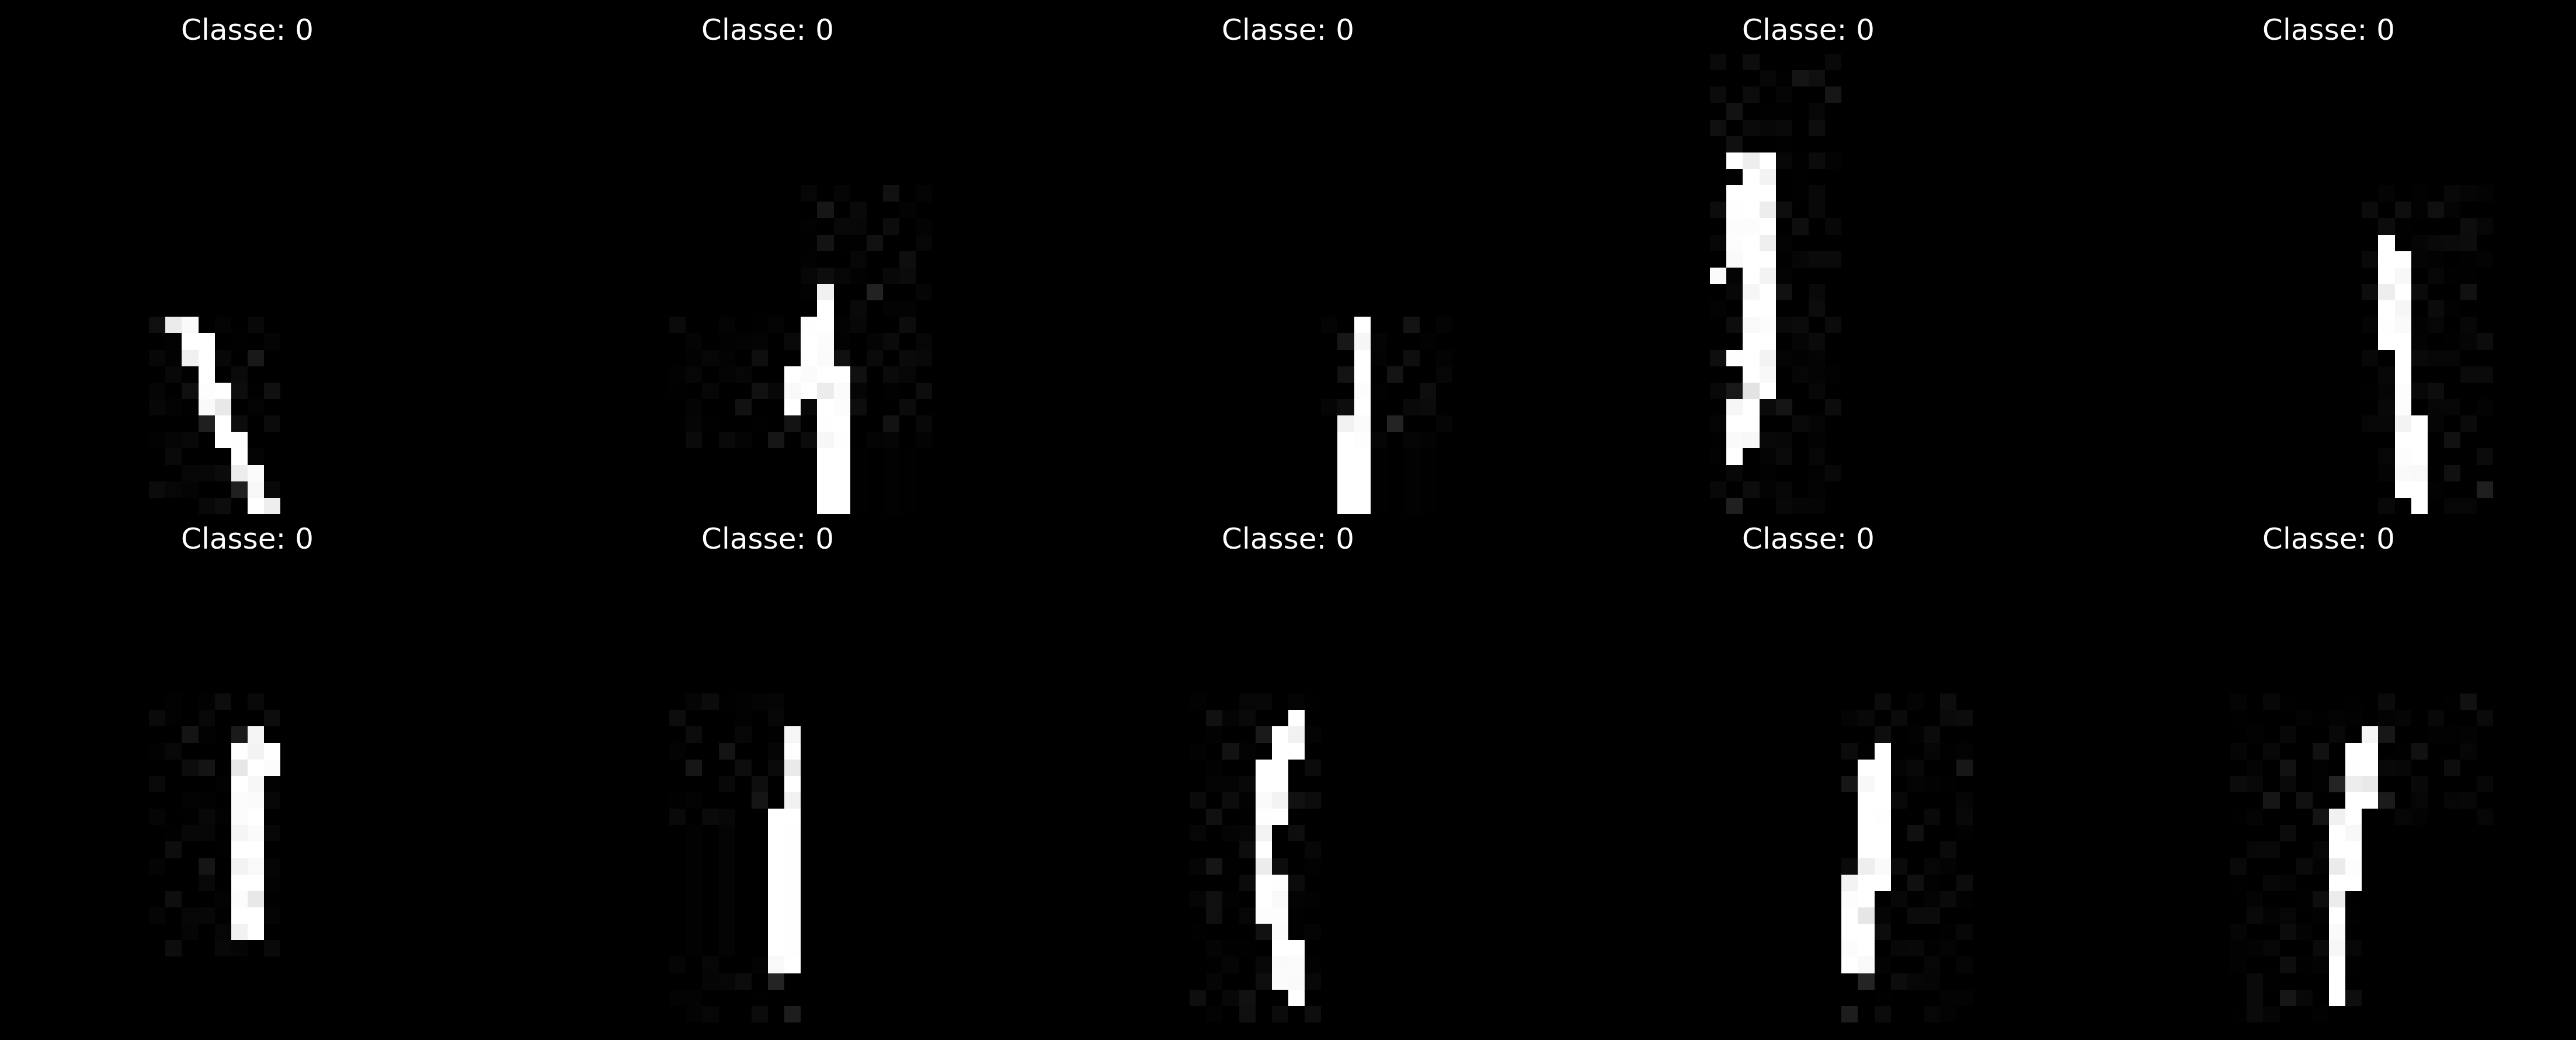
\includegraphics[width=\textwidth]{figures/urdu_examples.png}
                \caption{Exemples de caractères ourdou}
            \end{figure}
        \end{column}
    \end{columns}
\end{frame}

\section{Données et Défis}

\begin{frame}{Présentation des Données}
    \begin{columns}[T]
        \begin{column}{0.5\textwidth}
            \textbf{Structure du Dataset :}
            \begin{itemize}
                \item \textbf{Entraînement :} 28,328 images
                \item \textbf{Test :} 4,880 images
                \item \textbf{Classes :} 40 caractères distincts
                \item \textbf{Format :} 28×28 pixels (784 features)
            \end{itemize}
            
            \vspace{0.5cm}
            \textbf{Distribution des Classes :}
            \begin{itemize}
                \item Moyenne : \emphasize{708 échantillons/classe}
                \item Min : 512 (classe 26)
                \item Max : 829 (classe 4)
                \item Écart-type : 95 échantillons
            \end{itemize}
        \end{column}
        \begin{column}{0.5\textwidth}
            \begin{figure}
                \centering
                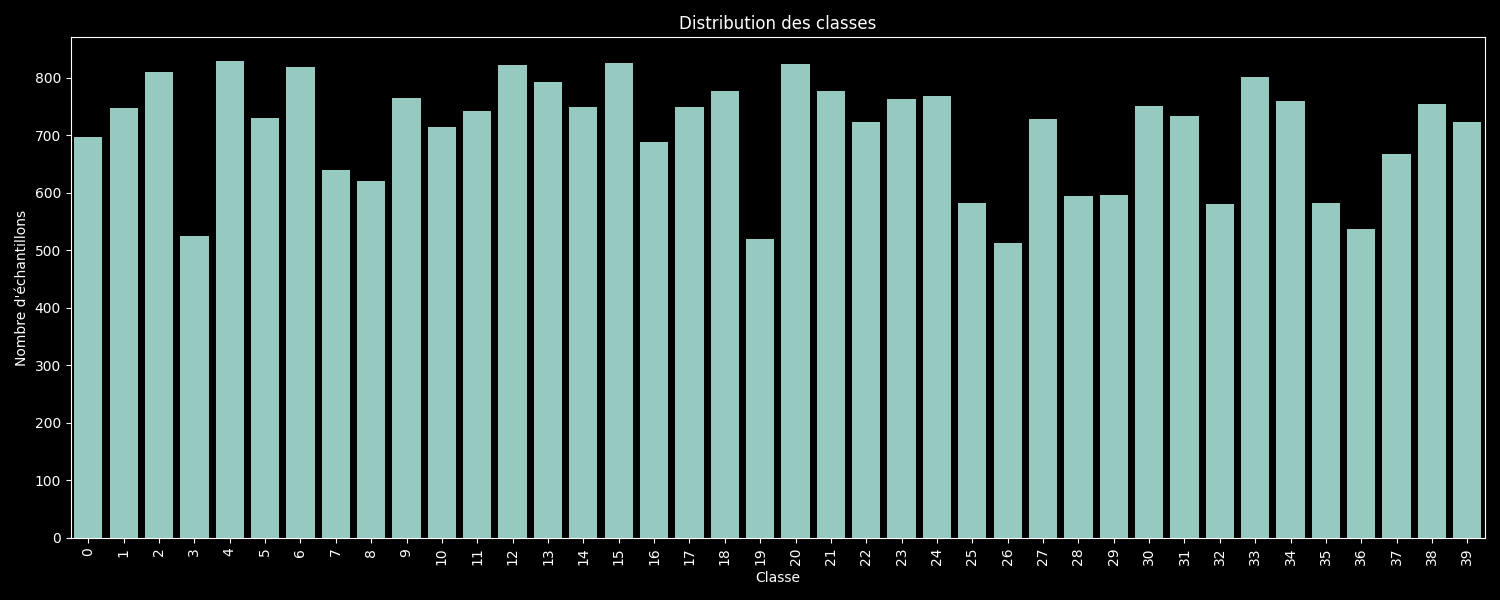
\includegraphics[width=\textwidth]{figures/class_distribution.png}
                \caption{Distribution des classes}
            \end{figure}
        \end{column}
    \end{columns}
\end{frame}

\begin{frame}{Défis Spécifiques de l'Ourdou}
    \begin{columns}[T]
        \begin{column}{0.6\textwidth}
            \textbf{Complexité Morphologique :}
            \begin{itemize}
                \item Formes curvilignes complexes
                \item Traits variables en épaisseur et orientation
                \item Structures calligraphiques élaborées
            \end{itemize}
            
            \vspace{0.3cm}
            \textbf{Similarité entre Caractères :}
            \begin{itemize}
                \item Différences subtiles (points diacritiques)
                \item Variations de courbes minimales
                \item Confusions potentielles fréquentes
            \end{itemize}
            
            \vspace{0.3cm}
            \textbf{Contraintes Techniques :}
            \begin{itemize}
                \item Résolution limitée (28×28)
                \item Variabilité stylistique
                \item Qualité d'image variable
            \end{itemize}
        \end{column}
        \begin{column}{0.4\textwidth}
            \begin{figure}
                \centering
                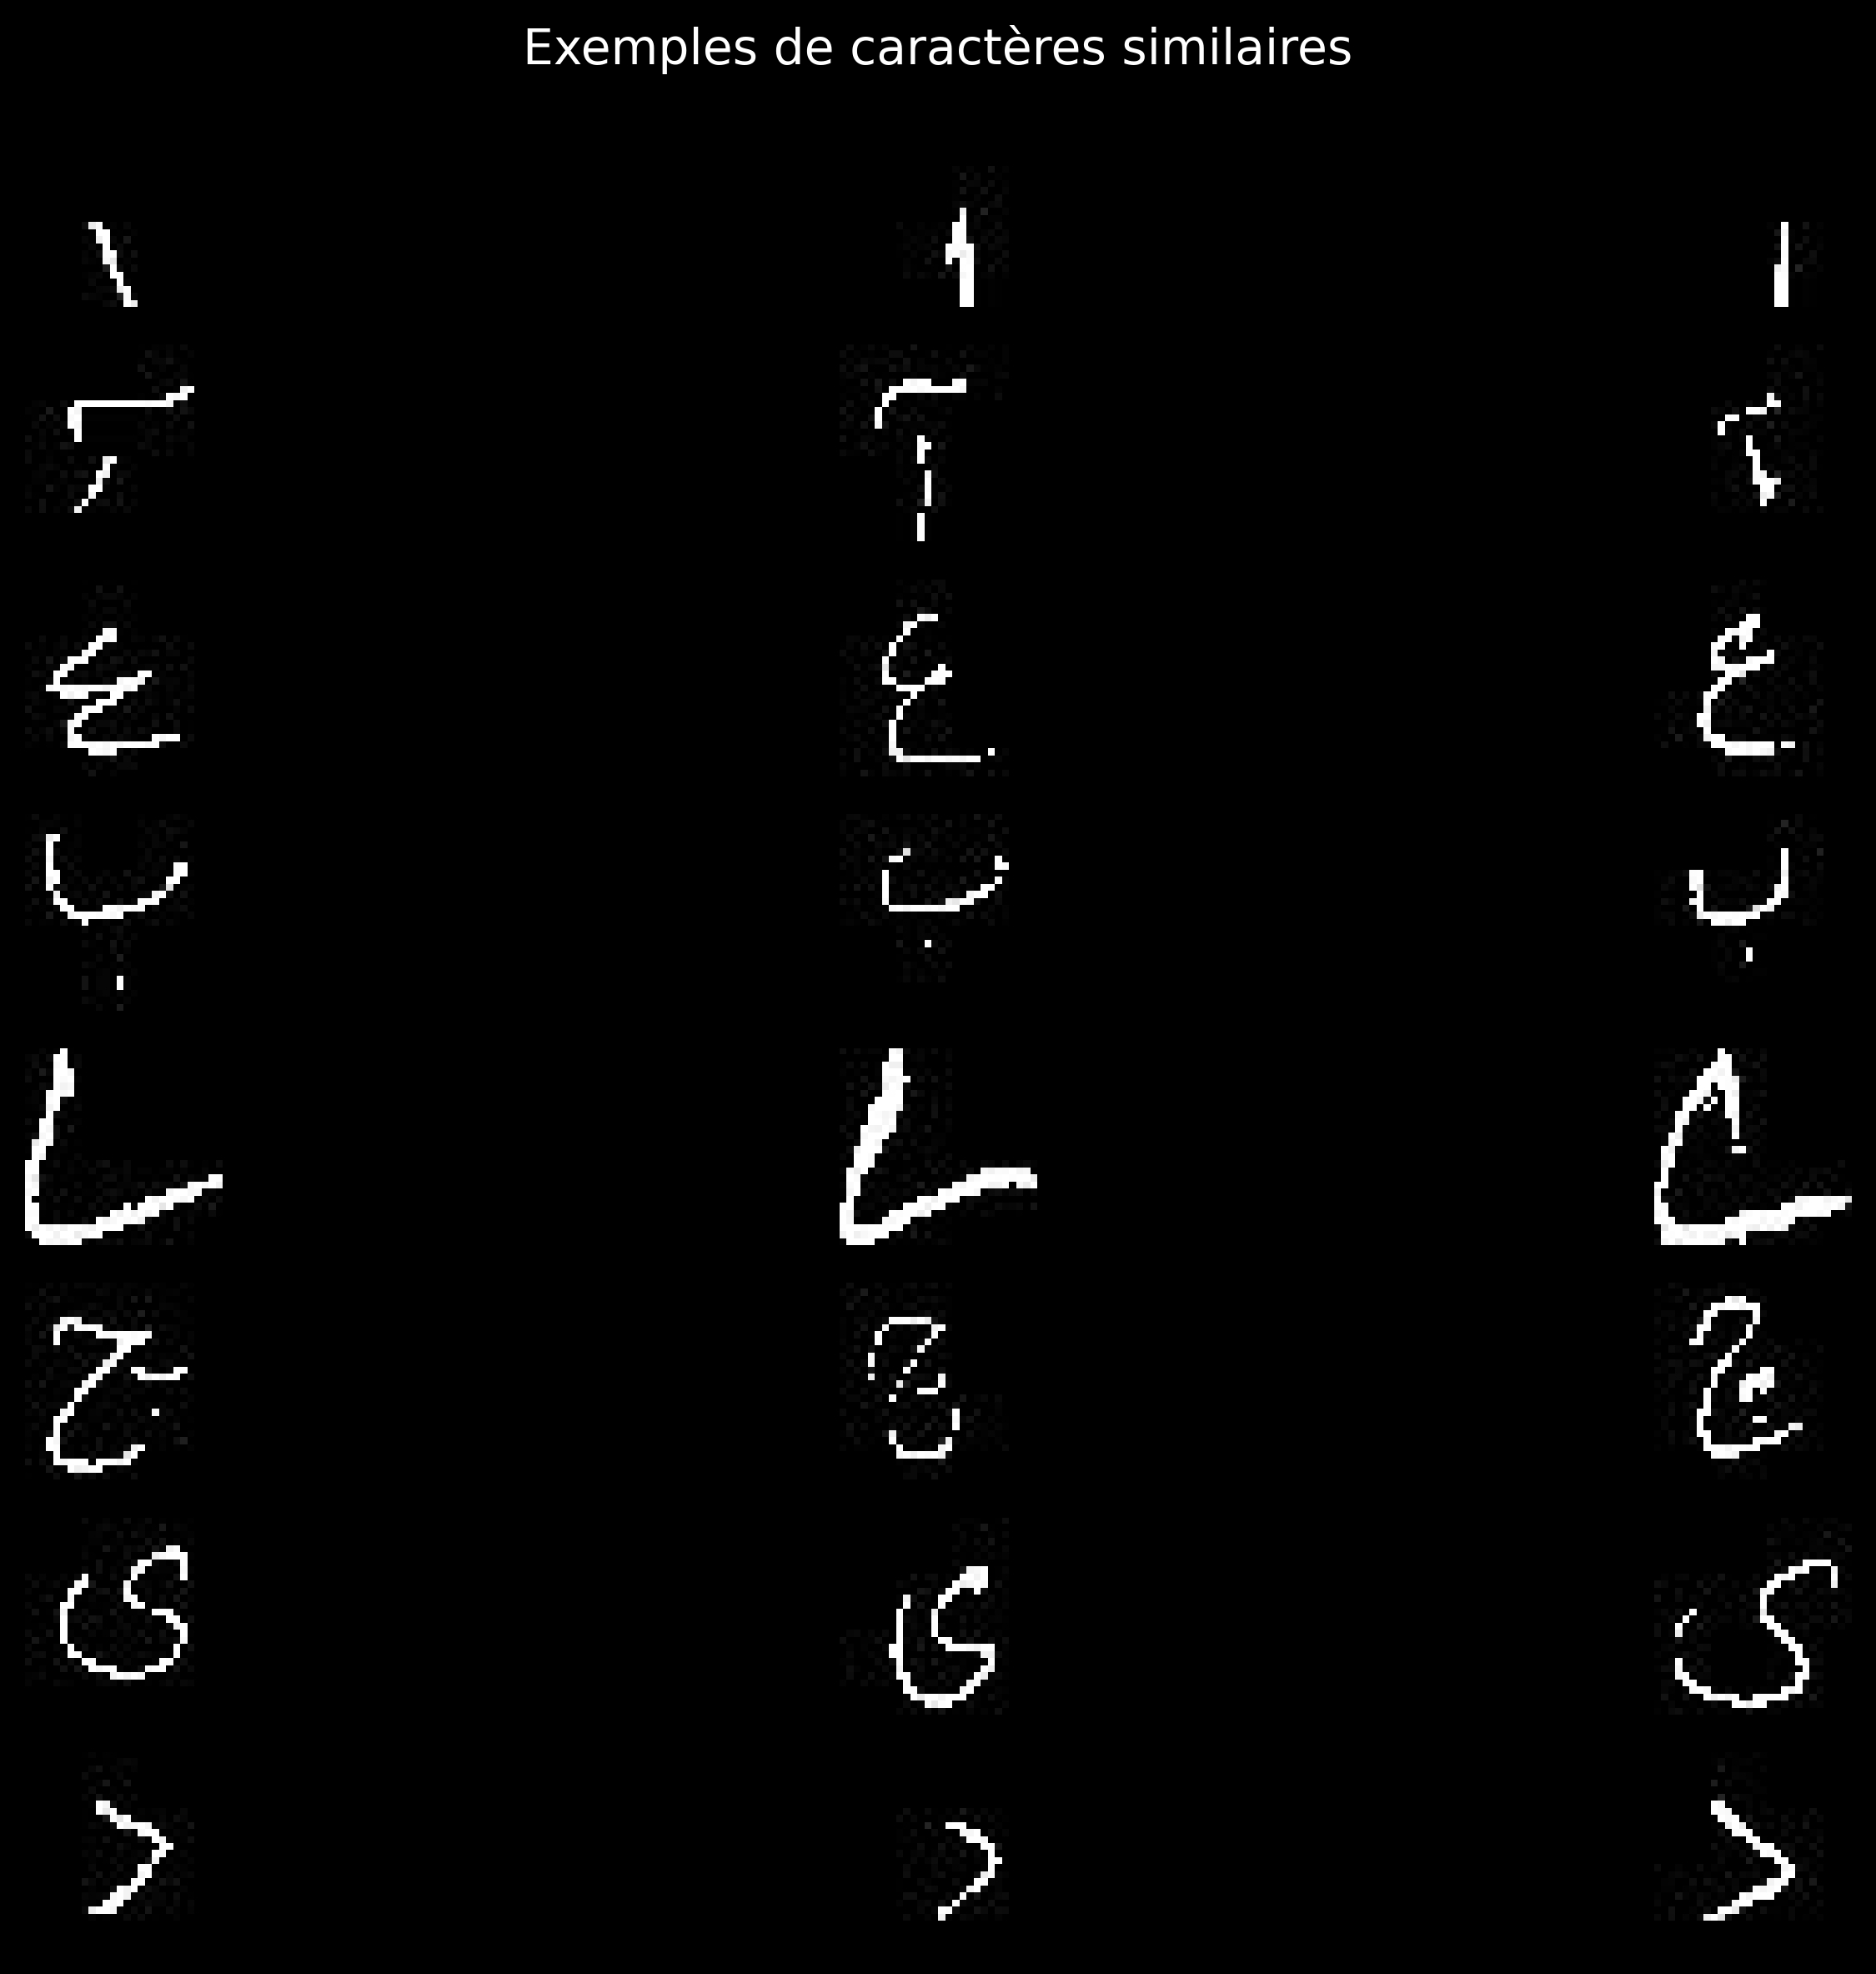
\includegraphics[width=\textwidth]{figures/similar_characters.png}
                \caption{Exemples de caractères similaires}
            \end{figure}
        \end{column}
    \end{columns}
\end{frame}

\section{Méthodologie Progressive}

\begin{frame}{Approche Méthodologique}
    \begin{center}
        \begin{tikzpicture}[node distance=3cm, auto]
            % Nodes
            \node[draw, rectangle, fill=univ_blue!20, text width=2.5cm, text centered] (mlp) {
                \textbf{MLP Simple} \\
                \small Baseline \\
                \small 543k paramètres
            };
            \node[draw, rectangle, fill=tech_green!20, text width=2.5cm, text centered, right of=mlp] (cnn) {
                \textbf{CNN Simple} \\
                \small Spatial \\
                \small 200k paramètres
            };
            \node[draw, rectangle, fill=accent_orange!20, text width=2.5cm, text centered, right of=cnn] (deep) {
                \textbf{CNN Profond} \\
                \small Avancé \\
                \small 447k paramètres
            };
            
            % Arrows
            \draw[->, thick] (mlp) -- (cnn) node[midway, above] {\small +Convolution};
            \draw[->, thick] (cnn) -- (deep) node[midway, above] {\small +Profondeur};
            
            % Results
            \node[below of=mlp, node distance=1.5cm] {\accuracy{54.6\%}};
            \node[below of=cnn, node distance=1.5cm] {\accuracy{88.4\%}};
            \node[below of=deep, node distance=1.5cm] {\accuracy{98.5\%}};
        \end{tikzpicture}
    \end{center}
    
    \vspace{0.5cm}
    \begin{center}
        \textbf{Progression logique :} Complexité croissante adaptée aux données image
    \end{center}
\end{frame}

\section{Résultats et Comparaisons}

\begin{frame}{Modèle 1 : MLP Simple}
    \begin{columns}[T]
        \begin{column}{0.5\textwidth}
            \textbf{Architecture :}
            \begin{itemize}
                \item Input(784) → Dense(512)
                \item Dense(256) → Output(40)
                \item Dropout (0.2), ReLU, Softmax
            \end{itemize}
            
            \vspace{0.3cm}
            \textbf{Résultats :}
            \begin{itemize}
                \item \accuracy{Précision : 54.6\%}
                \item Convergence dès l'époque 1
                \item Surapprentissage rapide
            \end{itemize}
            
            \vspace{0.3cm}
            \textbf{Limitations :}
            \begin{itemize}
                \item Perte information spatiale
                \item Sensibilité à la position
                \item Confusion entre caractères similaires
            \end{itemize}
        \end{column}
        \begin{column}{0.5\textwidth}
            \begin{figure}
                \centering
                
\includegraphics[width=\textwidth]{figures/mlp_training_history.png}
                \caption{Courbes d'apprentissage MLP}
            \end{figure}
            
            \begin{figure}
                \centering
                
\includegraphics[width=0.8\textwidth]{figures/mlp_confusion_matrix.png}
                \caption{Matrice de confusion MLP}
            \end{figure}
        \end{column}
    \end{columns}
\end{frame}

\begin{frame}{Modèle 2 : CNN Simple}
    \begin{columns}[T]
        \begin{column}{0.5\textwidth}
            \textbf{Architecture :}
            \begin{itemize}
                \item Conv2D(32) → MaxPool
                \item Conv2D(64) → MaxPool
                \item Flatten → Dense(128) → Output(40)
            \end{itemize}
            
            \vspace{0.3cm}
            \textbf{Améliorations :}
            \begin{itemize}
                \item Préservation structure spatiale
                \item Détection motifs locaux
                \item Invariance partielle aux translations
            \end{itemize}
            
            \vspace{0.3cm}
            \textbf{Résultats :}
            \begin{itemize}
                \item \accuracy{Précision : 88.4\% (+33.8 points)}
                \item Progression stable (10-12 époques)
                \item Matrice de confusion focalisée
            \end{itemize}
        \end{column}
        \begin{column}{0.5\textwidth}
            \begin{figure}
                \centering
                
\includegraphics[width=\textwidth]{figures/cnn_training_history.png}
                \caption{Courbes d'apprentissage CNN}
            \end{figure}
            
            \begin{figure}
                \centering
                
\includegraphics[width=0.8\textwidth]{figures/cnn_confusion_matrix.png}
                \caption{Matrice de confusion CNN}
            \end{figure}
        \end{column}
    \end{columns}
\end{frame}

\begin{frame}{Modèle 3 : CNN Profond}
    \begin{columns}[T]
        \begin{column}{0.5\textwidth}
            \textbf{Architecture Avancée :}
            \begin{itemize}
                \item 3 blocs convolutionnels (32→64→128)
                \item BatchNormalization après chaque couche
                \item Dropout stratifié (0.25/0.5)
                \item Padding 'same'
            \end{itemize}
            
            \vspace{0.3cm}
            \textbf{Techniques de Régularisation :}
            \begin{itemize}
                \item \textbf{BatchNormalization :} Stabilisation
                \item \textbf{Dropout adaptatif :} Anti-surapprentissage
                \item \textbf{ReduceLROnPlateau :} Optimisation fine
            \end{itemize}
        \end{column}
        \begin{column}{0.5\textwidth}
            \begin{figure}
                \centering
                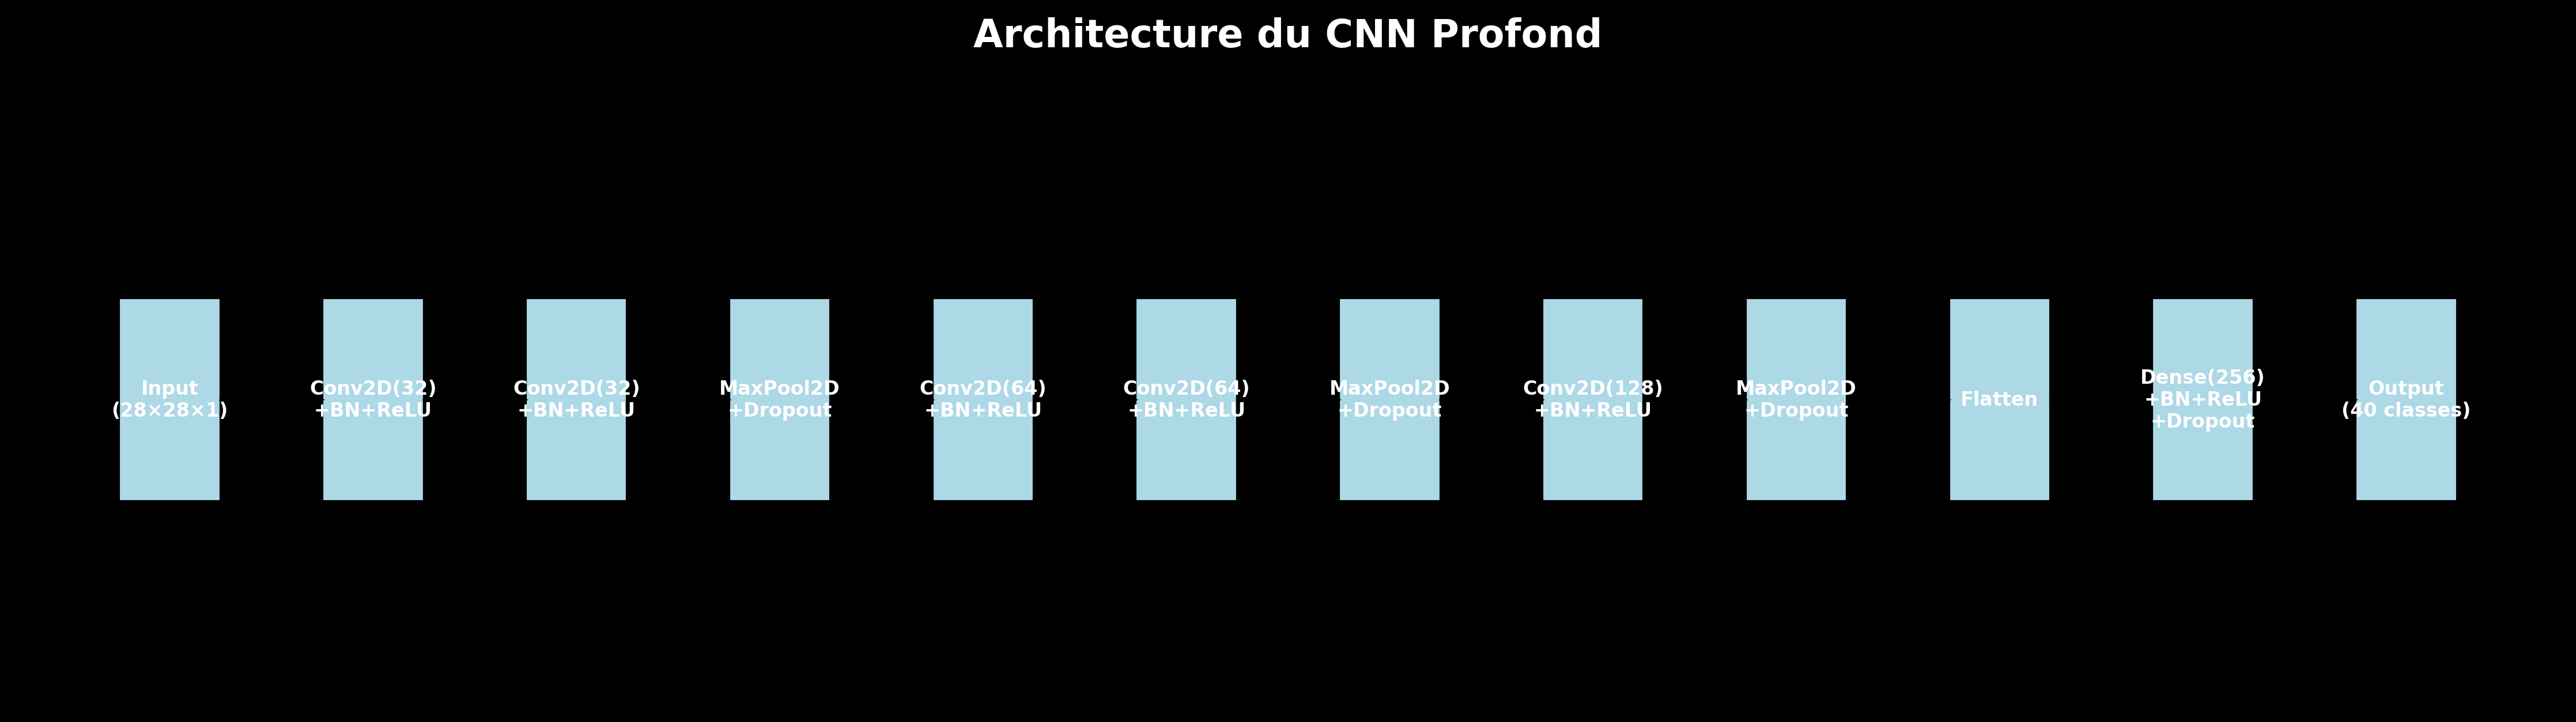
\includegraphics[width=\textwidth]{figures/cnn_architecture.png}
                \caption{Architecture CNN profond}
            \end{figure}
        \end{column}
    \end{columns}
\end{frame}

\begin{frame}{Résultats CNN Profond}
    \begin{columns}[T]
        \begin{column}{0.5\textwidth}
            \textbf{Performance Exceptionnelle :}
            \begin{itemize}
                \item \accuracy{Validation : 98.5\%}
                \item \accuracy{Test Kaggle : 99.1\%}
                \item Loss finale : 0.06
            \end{itemize}
            
            \vspace{0.3cm}
            \textbf{Caractéristiques :}
            \begin{itemize}
                \item Convergence stable (30 époques)
                \item Excellent équilibre train/validation
                \item Matrice de confusion quasi-diagonale
            \end{itemize}
            
            \vspace{0.3cm}
            \textbf{Erreurs Résiduelles :}
            \begin{itemize}
                \item Uniquement sur caractères très similaires
                \item Niveau quasi-humain
            \end{itemize}
        \end{column}
        \begin{column}{0.5\textwidth}
            \begin{figure}
                \centering
                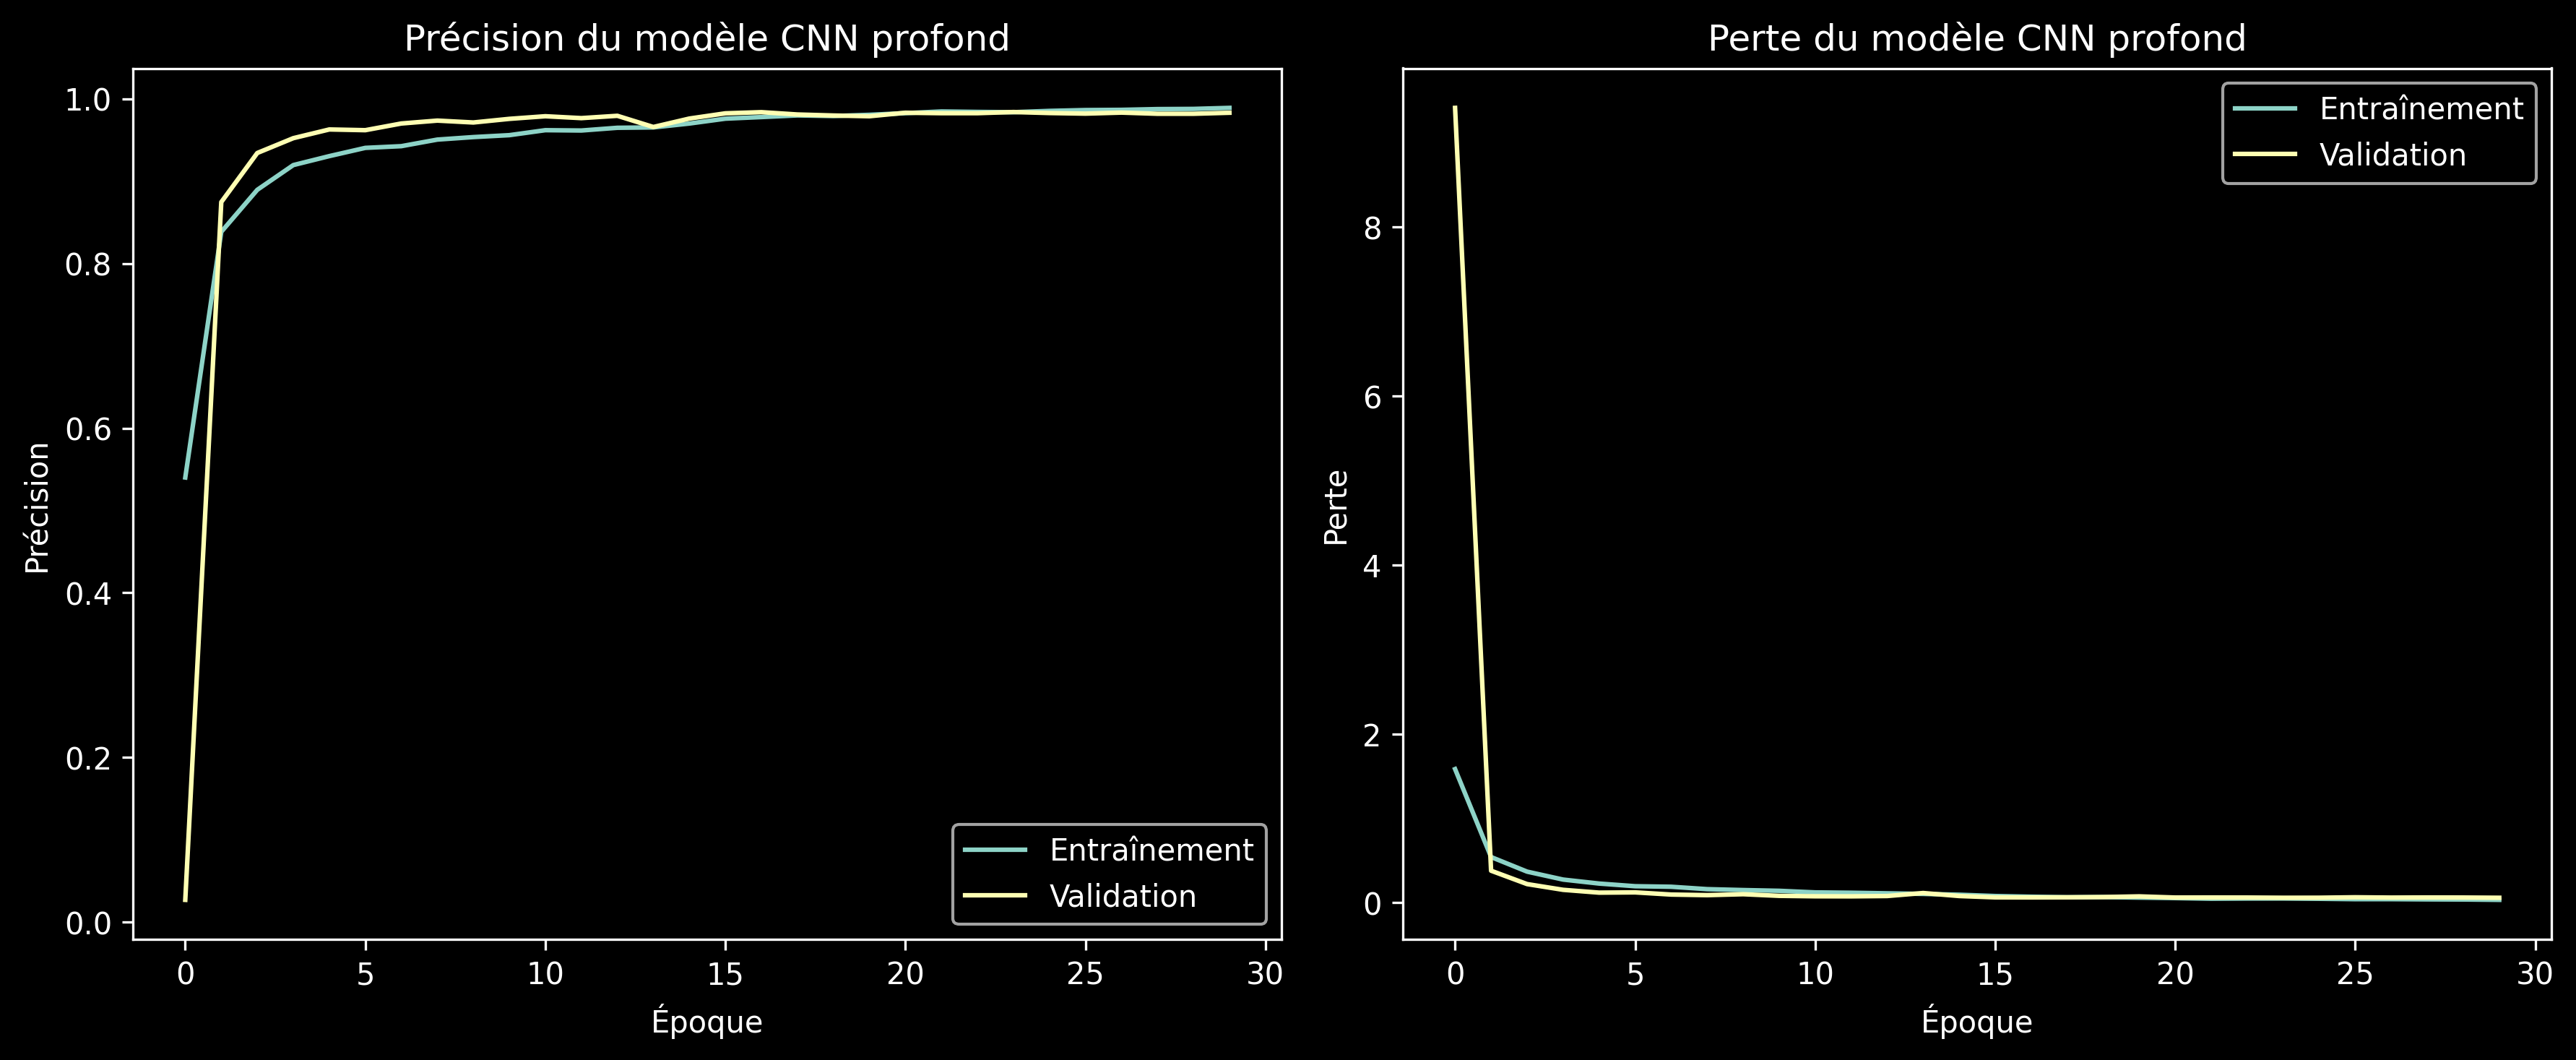
\includegraphics[width=\textwidth]{figures/deep_cnn_training_history.png}
                \caption{Courbes d'apprentissage CNN profond}
            \end{figure}
            
            \begin{figure}
                \centering
                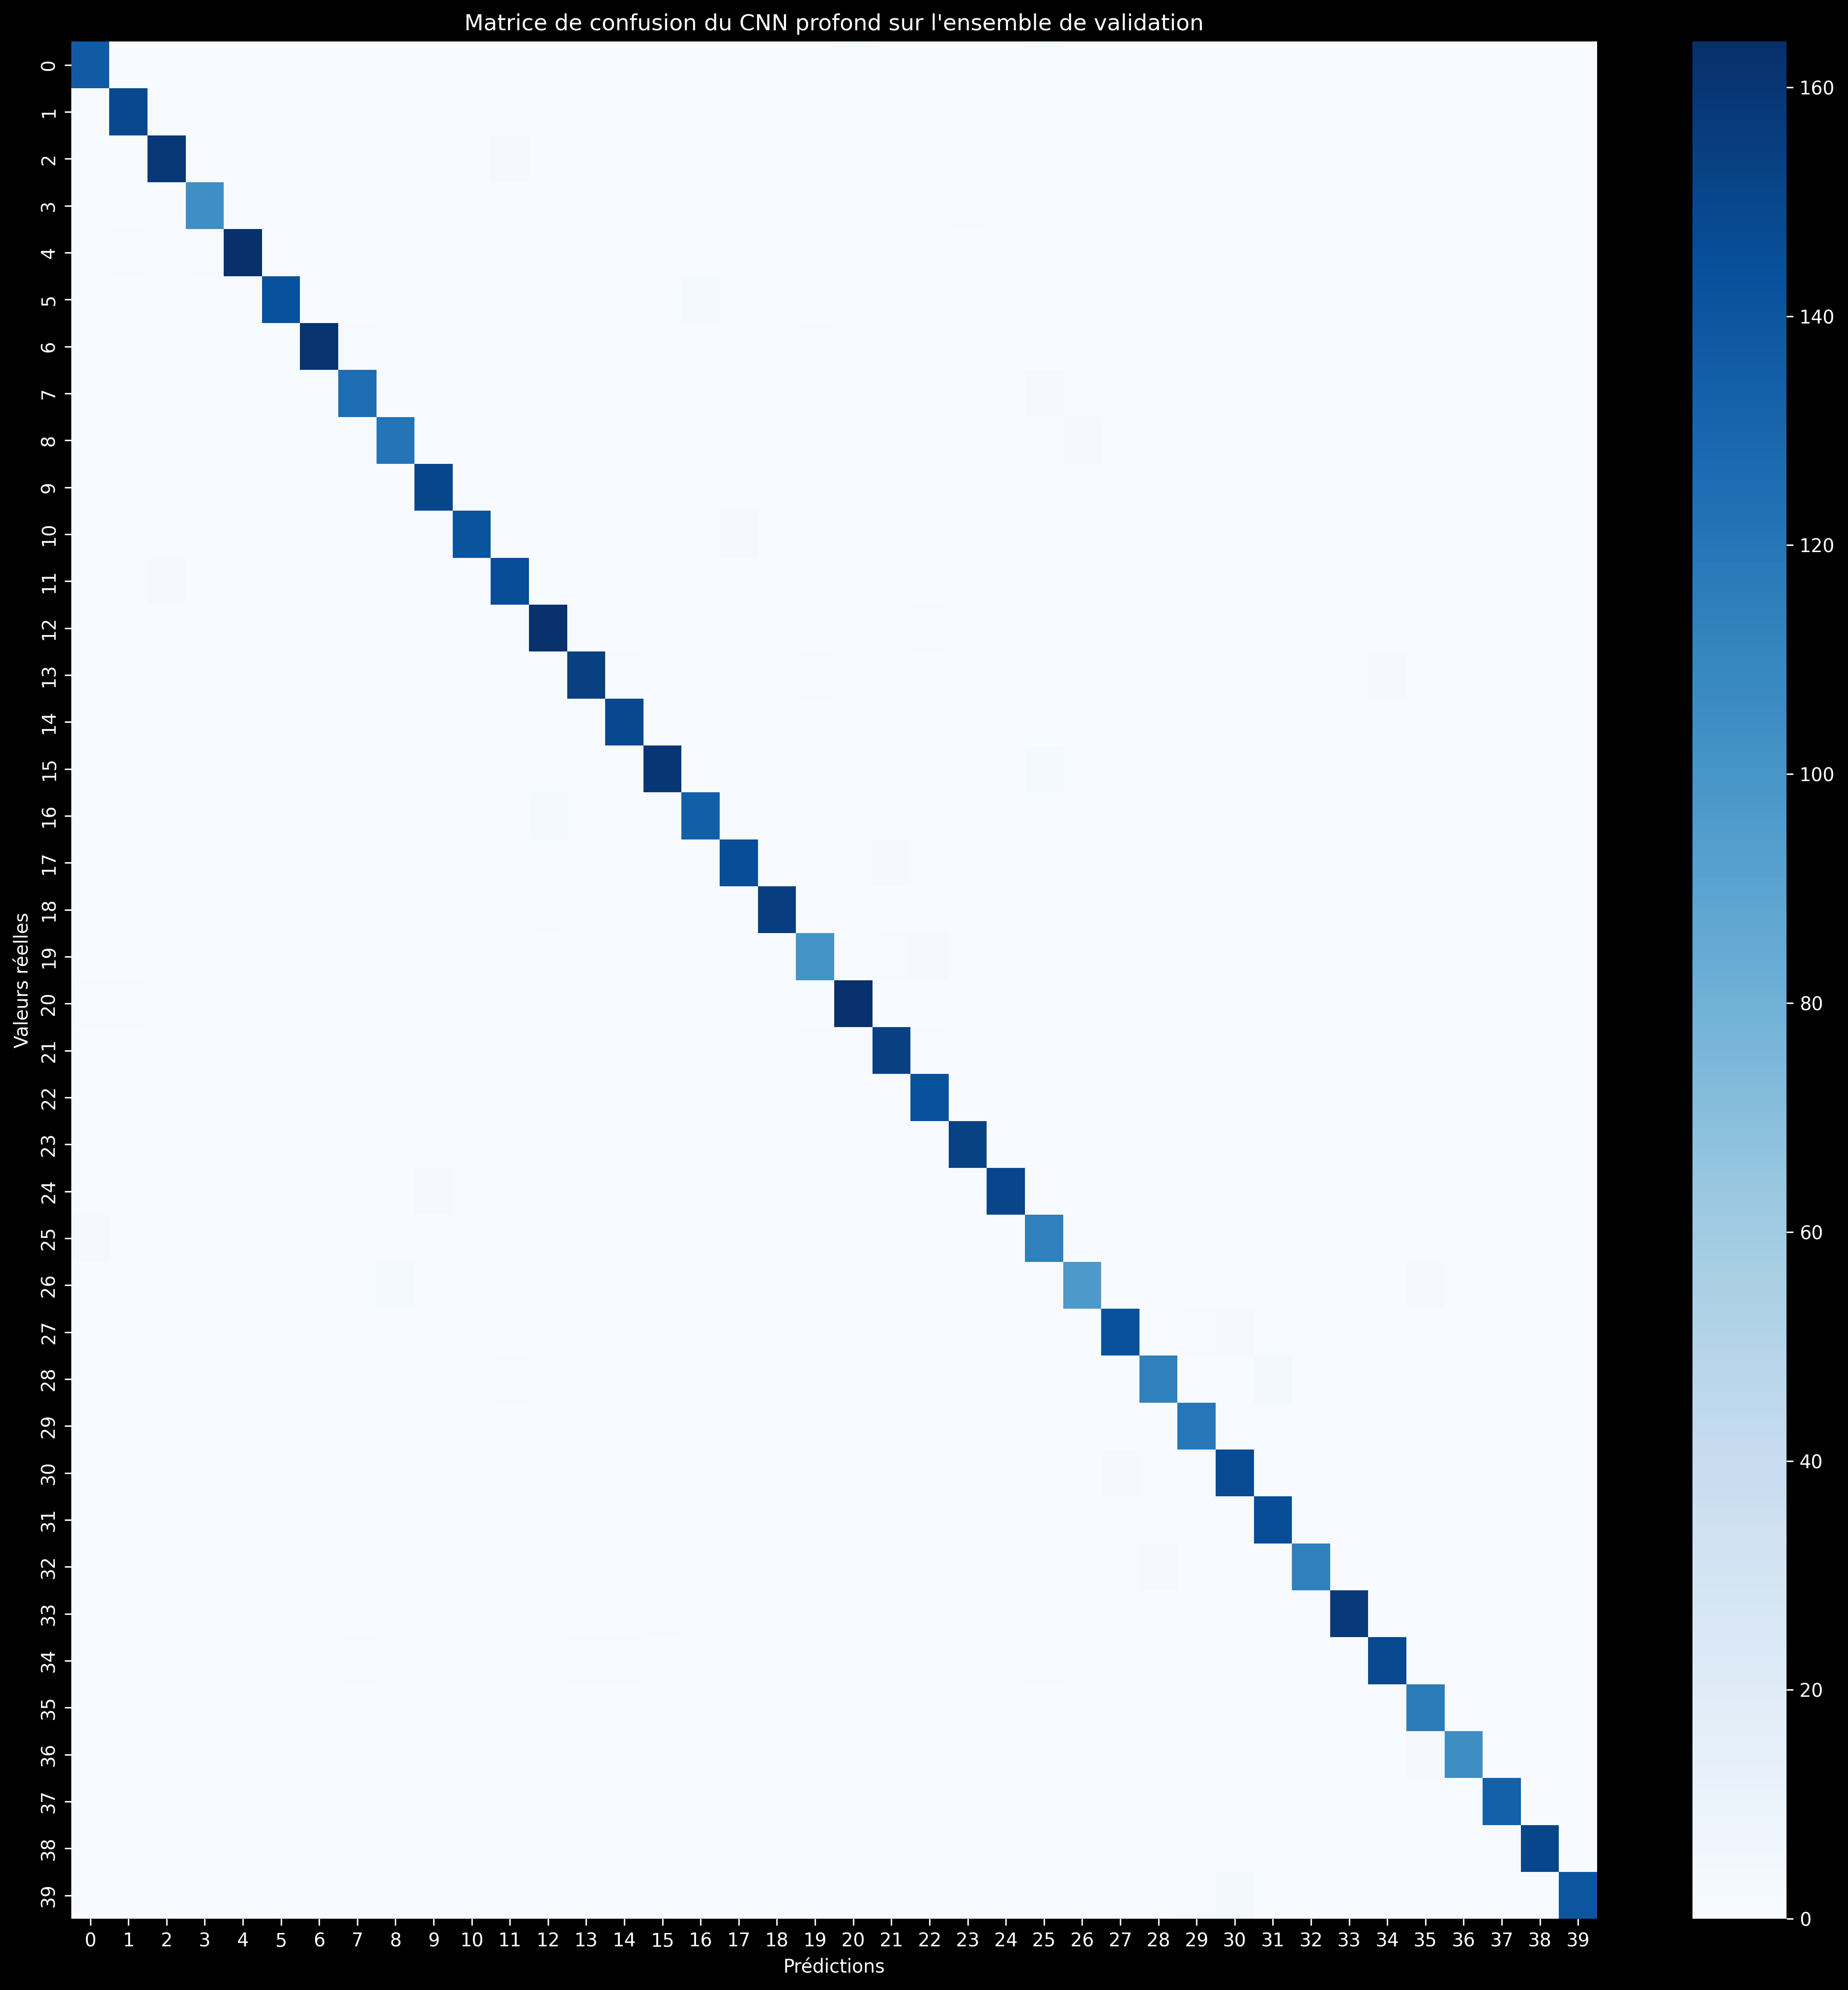
\includegraphics[width=0.8\textwidth]{figures/deep_cnn_confusion_matrix.png}
                \caption{Matrice de confusion optimale}
            \end{figure}
        \end{column}
    \end{columns}
\end{frame}

\section{Analyse et Perspectives}

\begin{frame}{Analyse Comparative}
    \begin{table}[h]
        \centering
        \begin{tabular}{@{}lcccc@{}}
            \toprule
            \textbf{Modèle} & \textbf{Précision} & \textbf{Paramètres} & \textbf{Temps} & \textbf{Époques} \\
            \midrule
            MLP Simple & \color{red}54.6\% & 537k & 4 min & 1 \\
            CNN Simple & \color{orange}88.4\% & 200k & 6 min & 11 \\
            CNN Profond & \color{tech_green}\textbf{98.5\%} & 447k & 15 min & 30 \\
            \bottomrule
        \end{tabular}
        \caption{Comparaison des performances}
    \end{table}
    
    \vspace{0.5cm}
    \begin{center}
        \emphasize{Gain total : +43.9 points de précision}
    \end{center}
    
    \vspace{0.3cm}
    \textbf{Facteurs clés d'amélioration :}
    \begin{itemize}
        \item Information spatiale préservée
        \item Hiérarchie de caractéristiques
        \item Régularisation avancée
        \item Optimisation adaptative
    \end{itemize}
\end{frame}

\begin{frame}{Évolution des Matrices de Confusion}
    \begin{figure}
        \centering
        \begin{minipage}{0.3\textwidth}
            \centering
            
\includegraphics[width=\textwidth]{figures/mlp_confusion_matrix.png}
            \caption{MLP - Confusion dispersée}
        \end{minipage}%
        \begin{minipage}{0.3\textwidth}
            \centering
            
\includegraphics[width=\textwidth]{figures/cnn_confusion_matrix.png}
            \caption{CNN - Confusions réduites}
        \end{minipage}%
        \begin{minipage}{0.3\textwidth}
            \centering
            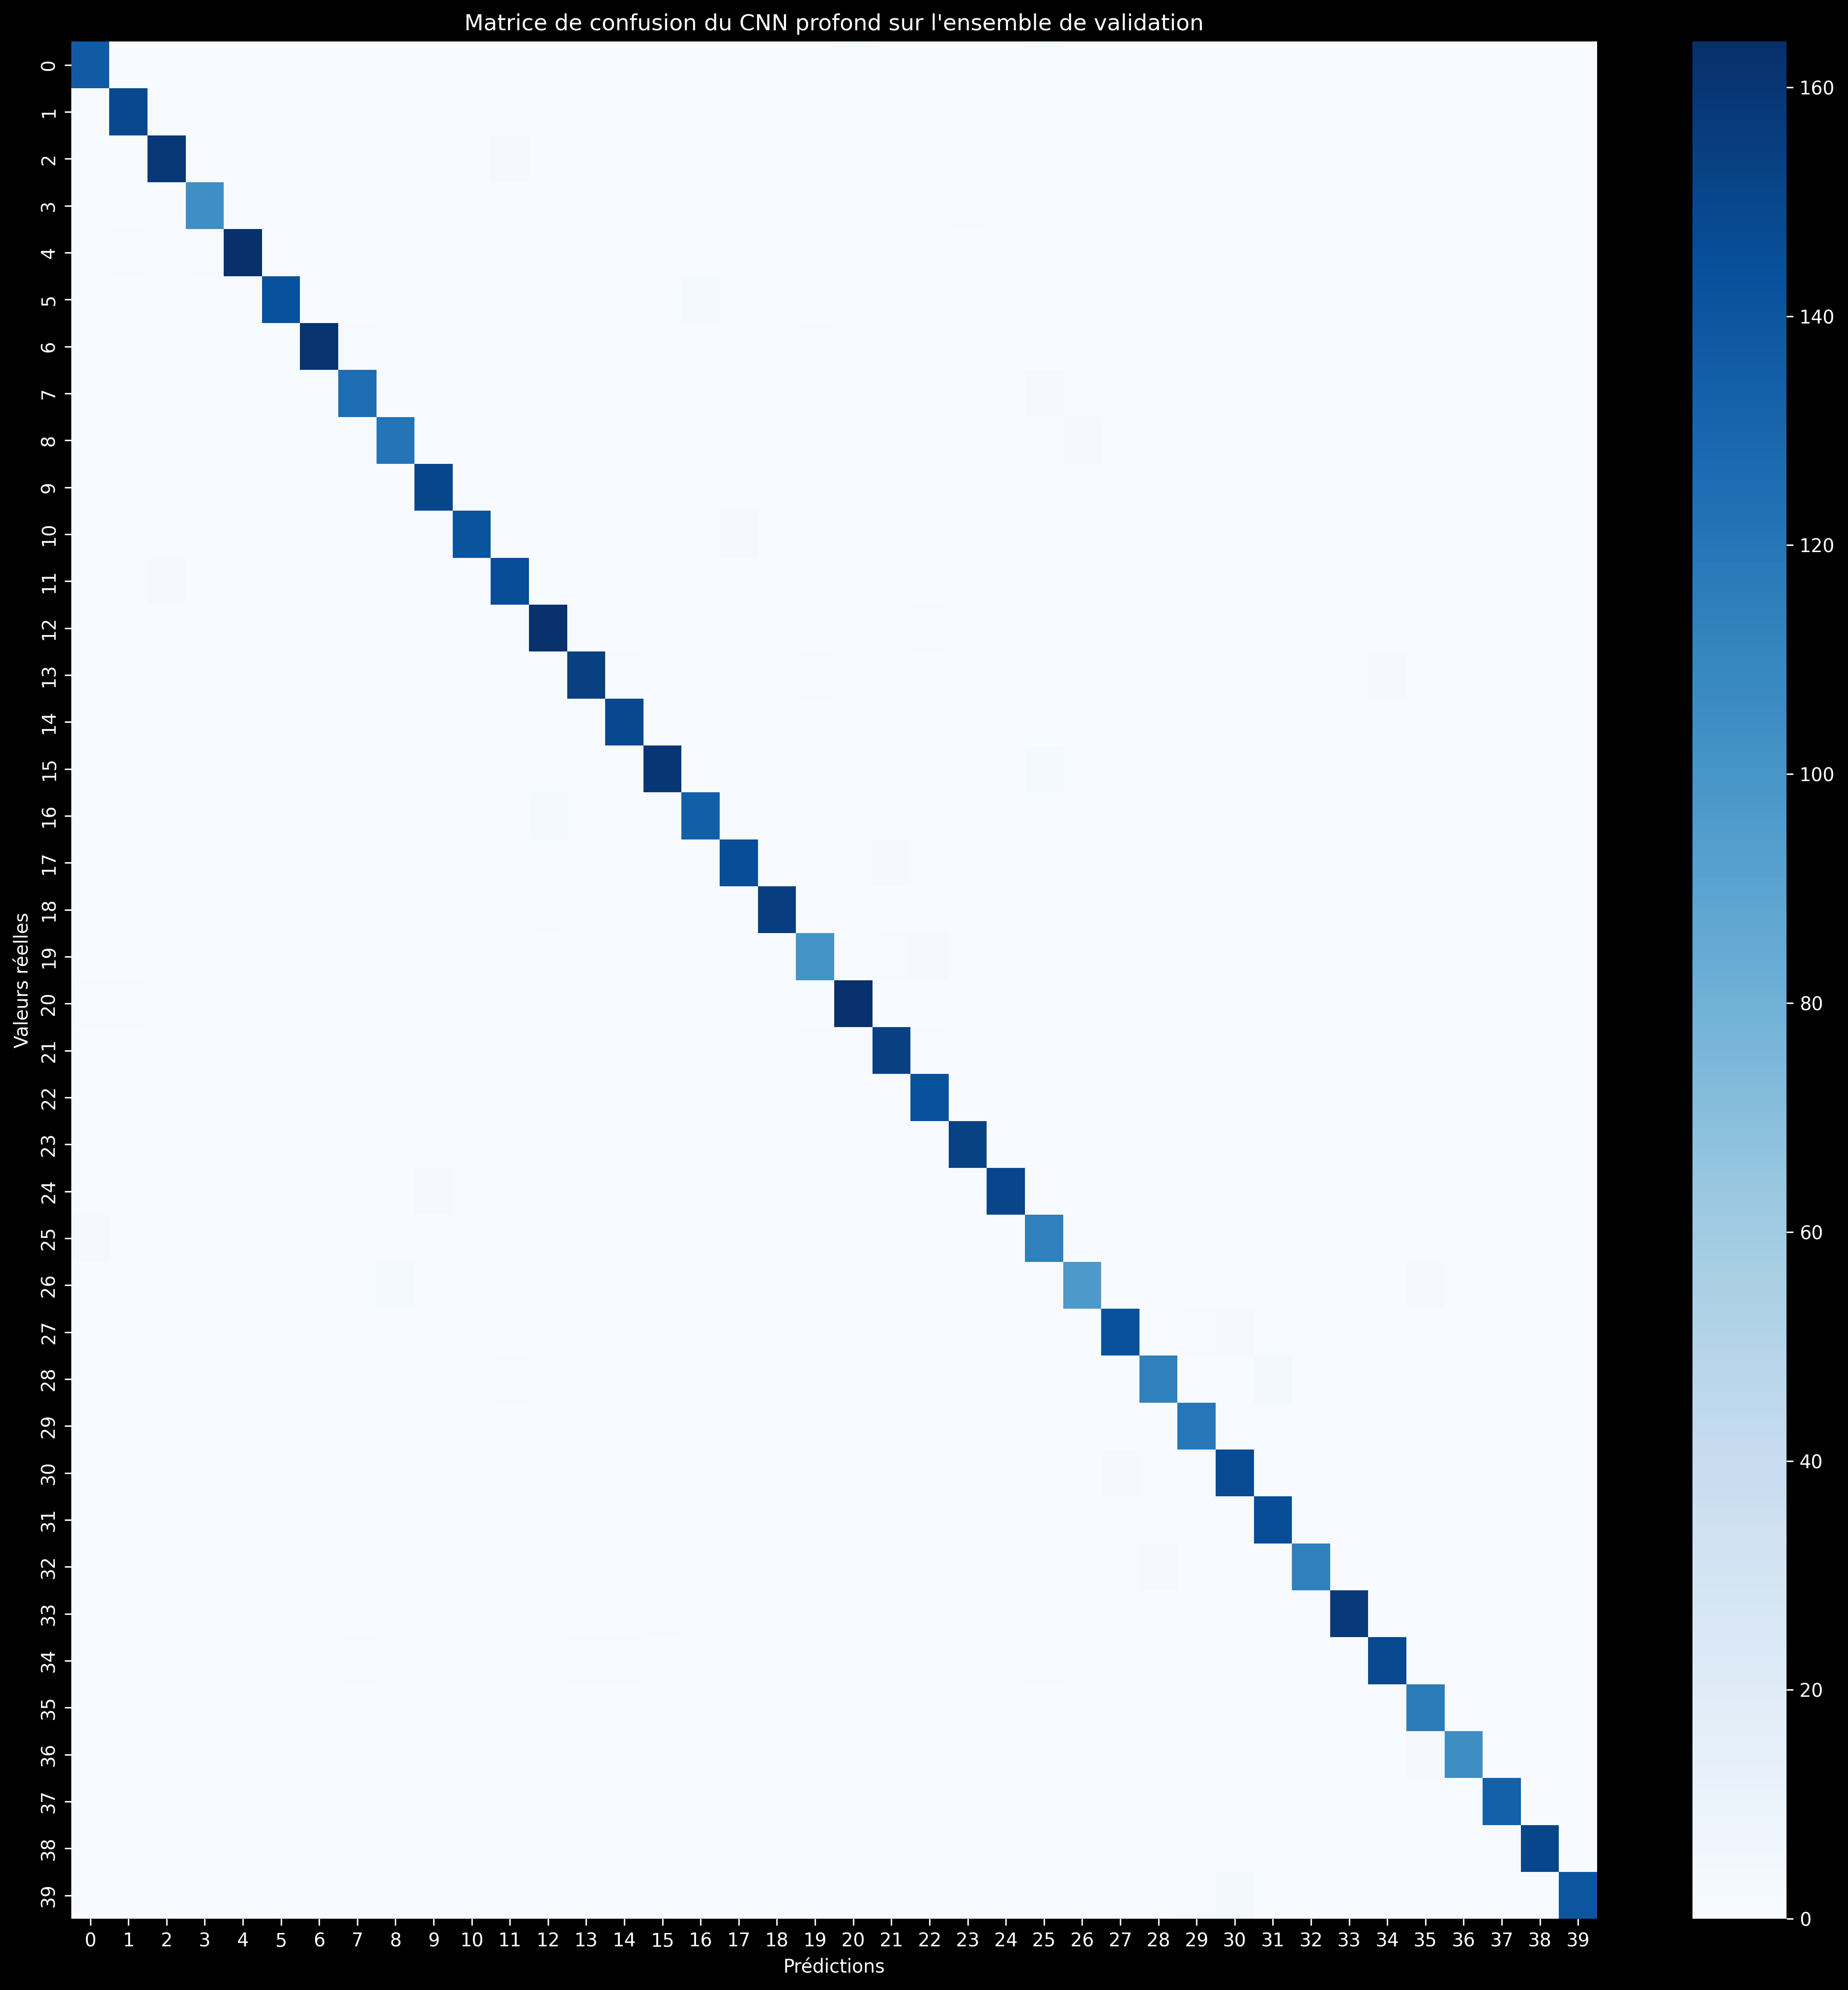
\includegraphics[width=\textwidth]{figures/deep_cnn_confusion_matrix.png}
            \caption{CNN Profond - Quasi-parfait}
        \end{minipage}
    \end{figure}
    
    \vspace{0.3cm}
    \begin{center}
        \textbf{Progression visible :} De la confusion dispersée à la diagonale dominante
    \end{center}
\end{frame}

\begin{frame}{Validation Kaggle}
    \begin{columns}[T]
        \begin{column}{0.6\textwidth}
            \textbf{Soumission Finale :}
            \begin{itemize}
                \item Score public : \accuracy{99.1\%}
                \item Cohérence avec validation locale (98.5\%)
                \item Excellente généralisation
            \end{itemize}
            
            \vspace{0.5cm}
            \textbf{Positionnement :}
            \begin{itemize}
                \item Parmi les meilleures performances
                \item Validation objective de l'approche
                \item Robustesse sur données inconnues
            \end{itemize}
            
            \vspace{0.5cm}
            \textbf{Validation de l'approche :}
            \begin{itemize}
                \item Méthodologie progressive efficace
                \item Choix architecturaux pertinents
                \item Optimisation technique réussie
            \end{itemize}
        \end{column}
        \begin{column}{0.4\textwidth}
            \begin{figure}
                \centering
                
\includegraphics[width=\textwidth]{figures/submission_preview.png}
                \caption{Aperçu soumission}
            \end{figure}
            
            \begin{figure}
                \centering
                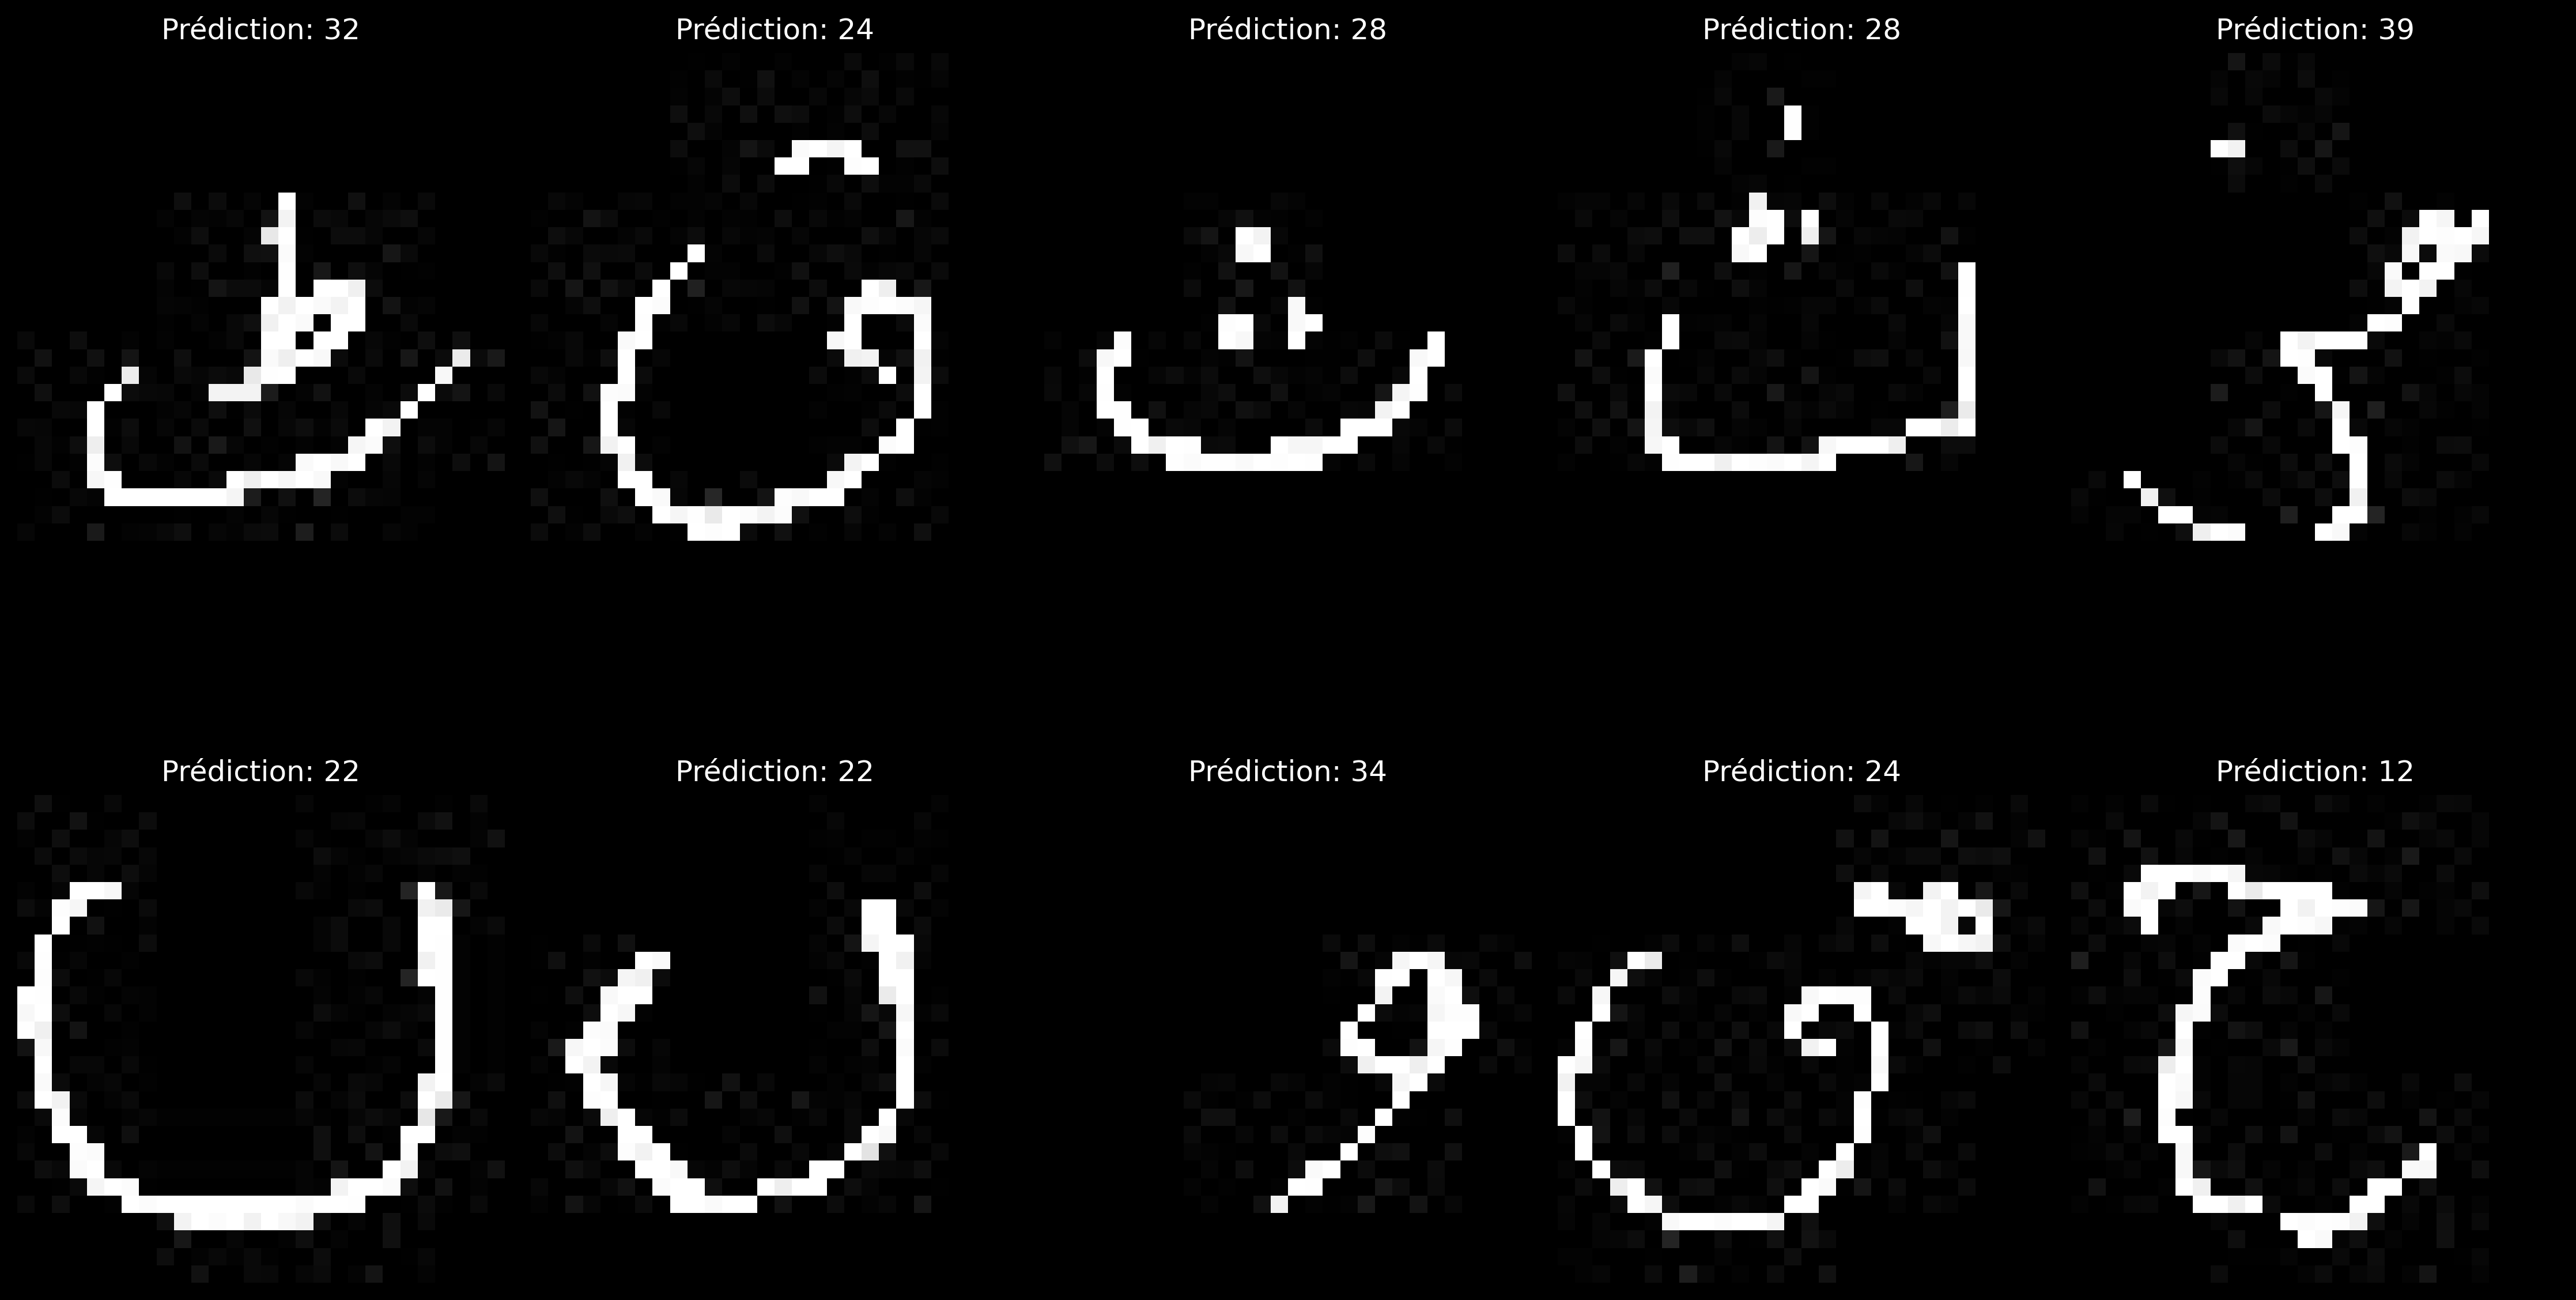
\includegraphics[width=\textwidth]{figures/prediction_examples.png}
                \caption{Exemples prédictions}
            \end{figure}
        \end{column}
    \end{columns}
\end{frame}

\begin{frame}{Perspectives et Améliorations}
    \begin{columns}[T]
        \begin{column}{0.5\textwidth}
            \textbf{Optimisations Possibles :}
            \begin{itemize}
                \item Recherche hyperparamètres systématique
                \item Augmentation de données (rotations, déformations)
                \item Régularisation avancée (Label smoothing, Mixup)
            \end{itemize}
            
            \vspace{0.3cm}
            \textbf{Architectures Avancées :}
            \begin{itemize}
                \item \textbf{ResNet :} Connexions résiduelles
                \item \textbf{Vision Transformers :} Mécanismes d'attention
                \item \textbf{Ensemble :} Combinaison de modèles
            \end{itemize}
        \end{column}
        \begin{column}{0.5\textwidth}
            \textbf{Applications Étendues :}
            \begin{itemize}
                \item OCR complet ourdou (segmentation + classification)
                \item Applications éducatives interactives
                \item Numérisation documents historiques
                \item Systèmes d'assistance multilingues
            \end{itemize}
            
            \vspace{0.3cm}
            \textbf{Impact Potentiel :}
            \begin{itemize}
                \item Préservation patrimoine numérique
                \item Accessibilité technologique
                \item Recherche en langues non-latines
            \end{itemize}
        \end{column}
    \end{columns}
\end{frame}

\section{Conclusion}

\begin{frame}{Conclusion}
    \textbf{Résultats Majeurs :}
    \begin{itemize}
        \item \emphasize{Progression spectaculaire :} 54.6\% → 99.1\%
        \item \emphasize{Validation méthodologique :} Importance architecture adaptée
        \item \emphasize{Performance exceptionnelle :} Niveau quasi-humain
    \end{itemize}
    
    \vspace{0.5cm}
    \textbf{Contributions :}
    \begin{itemize}
        \item \textbf{Académique :} Compréhension approfondie du Deep Learning
        \item \textbf{Technique :} Solution efficace pour caractères ourdou
        \item \textbf{Méthodologique :} Approche progressive reproductible
    \end{itemize}
    
    \vspace{0.5cm}
    \textbf{Impact :} Démonstration concrète du potentiel des CNN pour la préservation des langues non-latines
    
    \vspace{0.5cm}
    \begin{center}
        \Large \textcolor{tech_green}{\textbf{Merci pour votre attention !}}
    \end{center}
\end{frame}

\begin{frame}{Questions et Discussion}
    \begin{center}
        \Huge Questions ?
        
        \vspace{1cm}
        
        \Large
        \begin{itemize}
            \item Choix architecturaux
            \item Défis techniques rencontrés
            \item Applications futures
            \item Évolutions du projet
        \end{itemize}
    \end{center}
\end{frame}

\end{document}